\section{Introduction: The axial mass problem}
The axial-vector and pseudoscalar form-factors in the electroweak nucleon current are the subject of long-standing theoretical and experimental efforts. However, these values still remain rather poorly known. Within the framework of the conventional parametrizations, both form-factors are characterized by a single phenomenological parameter, nucleon axial mass $M_{A}$:
\begin{equation}
F_{P}(Q^{2})={}\frac{2M^{2}}{m_{\pi}^{2}+Q^{2}}F_{A}(Q^{2}),\\
F_{A}(Q^{2})={}g_{A}\left(1+\frac{Q^{2}}{M_{A}^{2}}\right)^{-2},
\end{equation}
here $g_{A}=-1.2695$ --- axial-vector coupling, $m_{\pi}$ --- charged pion mass, $M=(M_{n}+M_{p})/2$ --- isoscalar nucleon mass, $Q^{2}=-q^{2}$, where $q^{2}$ --- squared 4-momentum transfer~\cite{Kuzmin:2007kr}.

Global statistical analysis of all available and mutually consistent data on the total and differential cross sections for the $\nu_{\mu}$ and $\bar\nu_{\mu}$ quasielastic scattering (QES) on hydrogen and deuterium and also on different nuclear targets at high energies us to extract the best-fit value of nucleon axial mass: $M_{A}=1.012\pm0.031$\,GeV~\cite{Kuzmin:2014}. In Fig.~\ref{TotalCS} we demonstrate several examples of this analysis. The problem is in huge disagreement between the obtained best-fit value and the value extracted in the K2K and (especially) MiniBooNE experiments. Figures~\ref{K2K} and \ref{MiniBooNE} represent the K2K and the MiniBooNE measurements: $M_{A}=1.20\pm0.12$\,GeV~\cite{Gran:2006jn} and $M_{A}=1.35\pm0.17$\,GeV~\cite{AguilarArevalo:2010zc}, respectively. Thus, there is no consensus about right value of nucleon axial mass.

\begin{figure}[htb!]
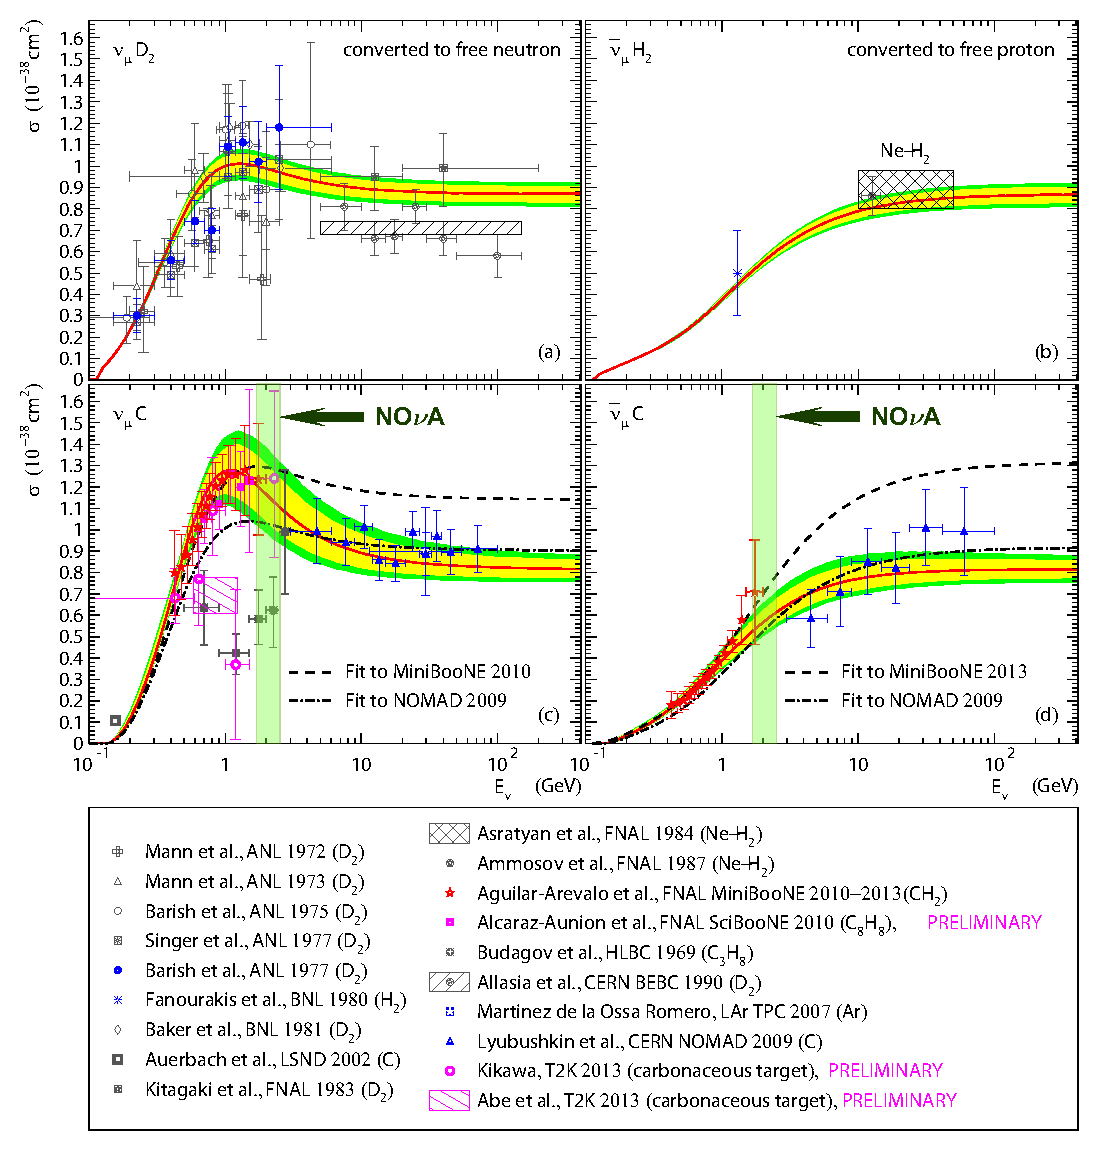
\includegraphics[width=0.5\textwidth]{./QES/sQESCC_101.2.31.301.1b_2_BBBA25_NT_1_NOvA.eps}
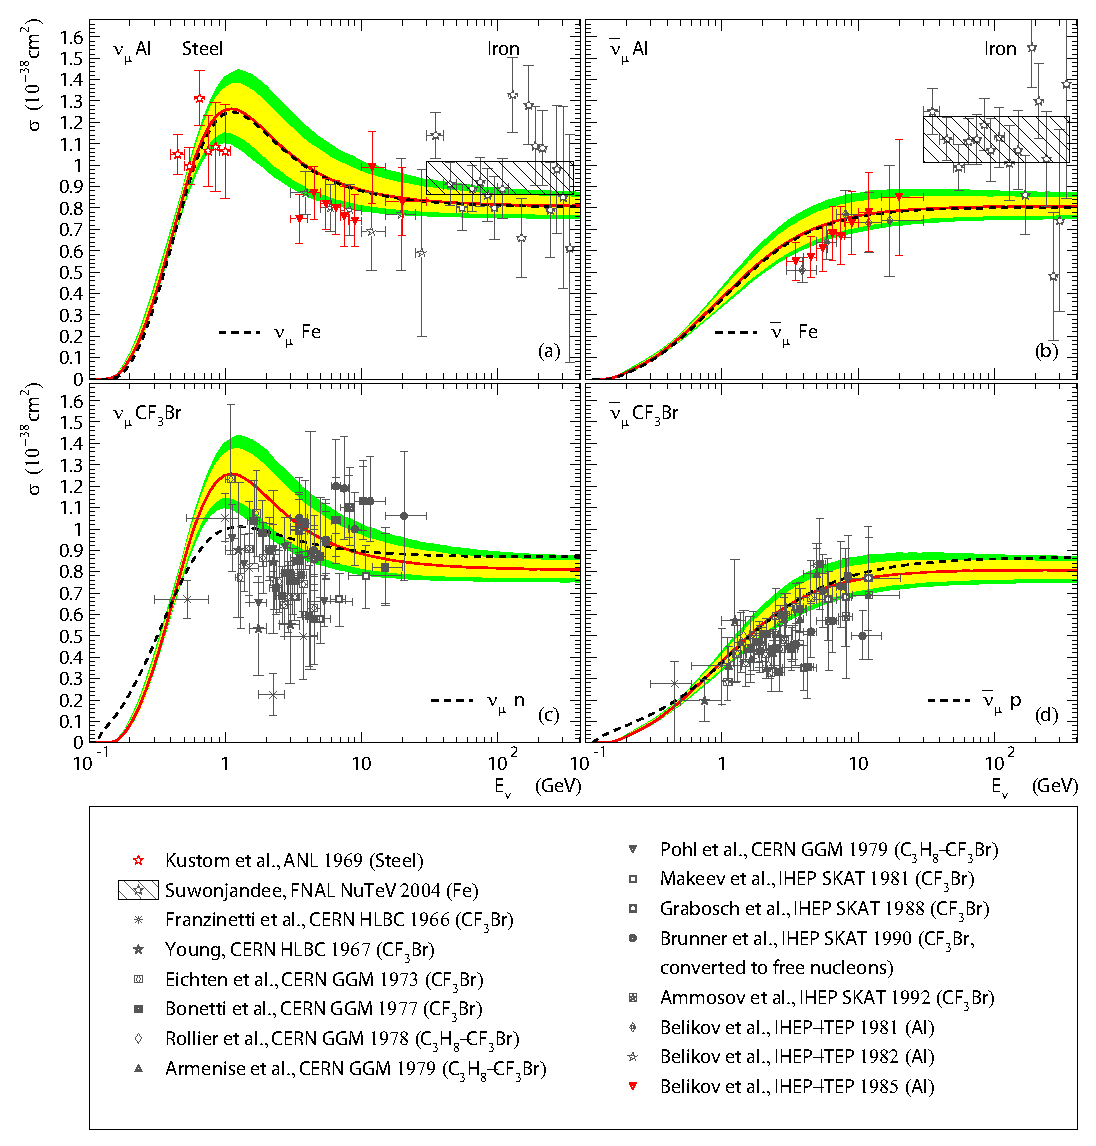
\includegraphics[width=0.5\textwidth]{./QES/sQESCC_101.2.31.301.1b_2_BBBA25_NT_2.eps}
\caption{\label{TotalCS}\textbf{Total QES $\nu_{\mu}n$ \& $\bar\nu_{\mu}p$ cross sections} measured in experiments with deuterium, hydrogen and other targets. The light points are excluded from the global fit being either superseded by newer experiments, or not satisfying our selection criteria (see Ref.\cite{Kuzmin:2007kr} for more details and for the full set of the experimental data). The dash-dotted curves show cross sections calculated with the NOMAD result: $M_A=1.05\pm0.02\pm0.06$\,GeV~\cite{Lyubushkin:2008pe}. The \textbf{dashed curves correspond} the MiniBooNE result: $M_{A}=1.35\pm0.17$\,GeV~\cite{AguilarArevalo:2010zc}. The solid curve represent the effective axial mass application. The widths of the inner (outer) bands correspond to the $1\sigma$ ($2\sigma$) standard deviations from the fit caused by the uncertainties in determination of $M_{A}$ including the spectrum normalizations}
\end{figure}

\begin{figure}[htb!]
\begin{center}
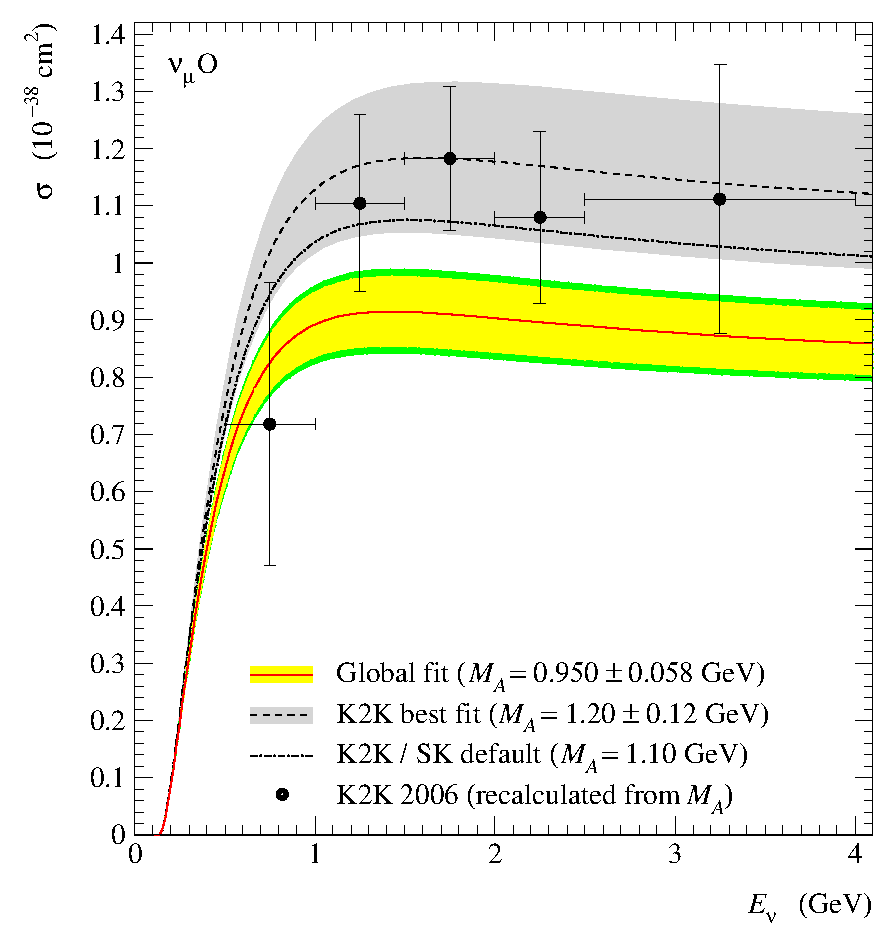
\includegraphics[width=0.45\textwidth]{./QES/sQESCC_K2K06_101.3.00.301.00_2_BBBA25_SM.eps}
\caption{\label{K2K}\textbf{A comparison of the QES $\nu_{\mu}$ cross sections} per neutron bound in oxygen evaluated with different values of $M_{A}$. The dashed curve with accompanying band corresponds to the K2K extraction of $M_{A}$~\cite{Gran:2006jn}. The dash-dotted curve is the cross section calculated with $M_{A}=1.1$\,GeV, the value which was the K2K and SK\,I default before 2006~\cite{Gran:2006jn,Ashie:2005ik}. The points in Fig.~\ref{K2K} represent the total QES cross section reconstructed from the ``raw'' K2K data}
\end{center}
\end{figure}

\begin{figure}[htb!]
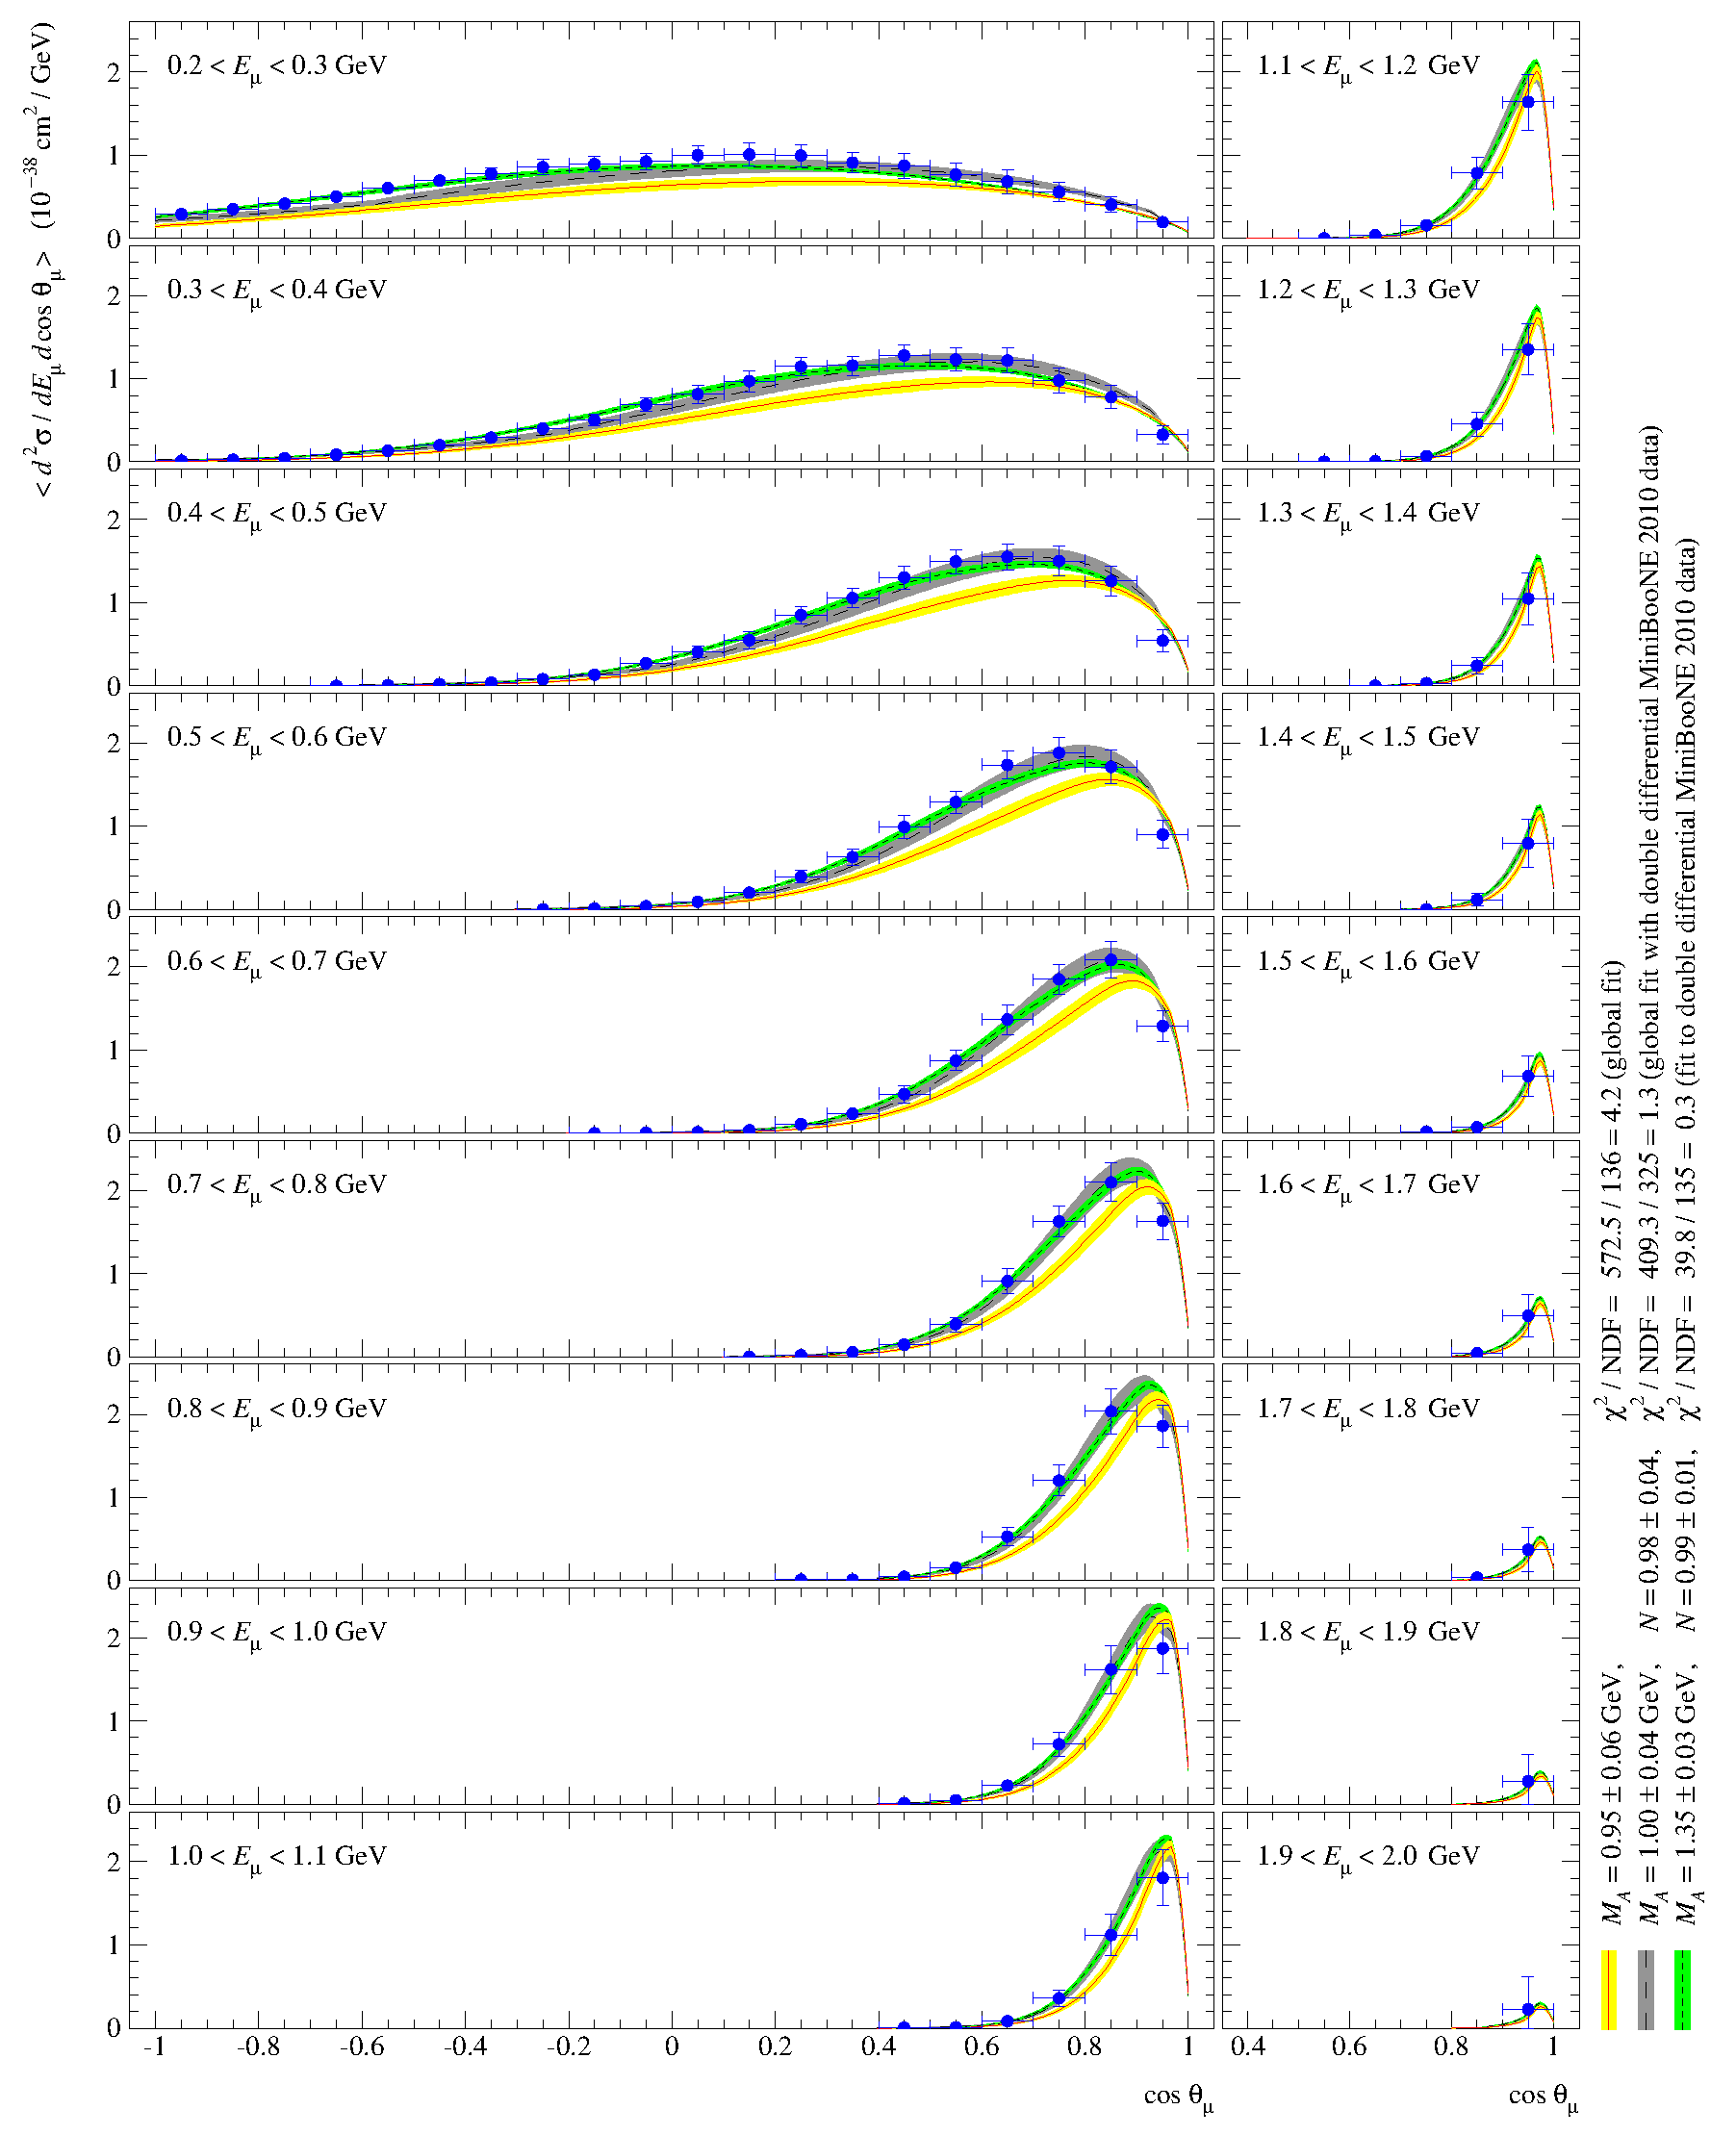
\includegraphics[width=0.5\textwidth]{./QES/d2sQESCC_dEkdcosT_Arevalo_MiniBooNE10_Ek_2_BBBA25.eps}
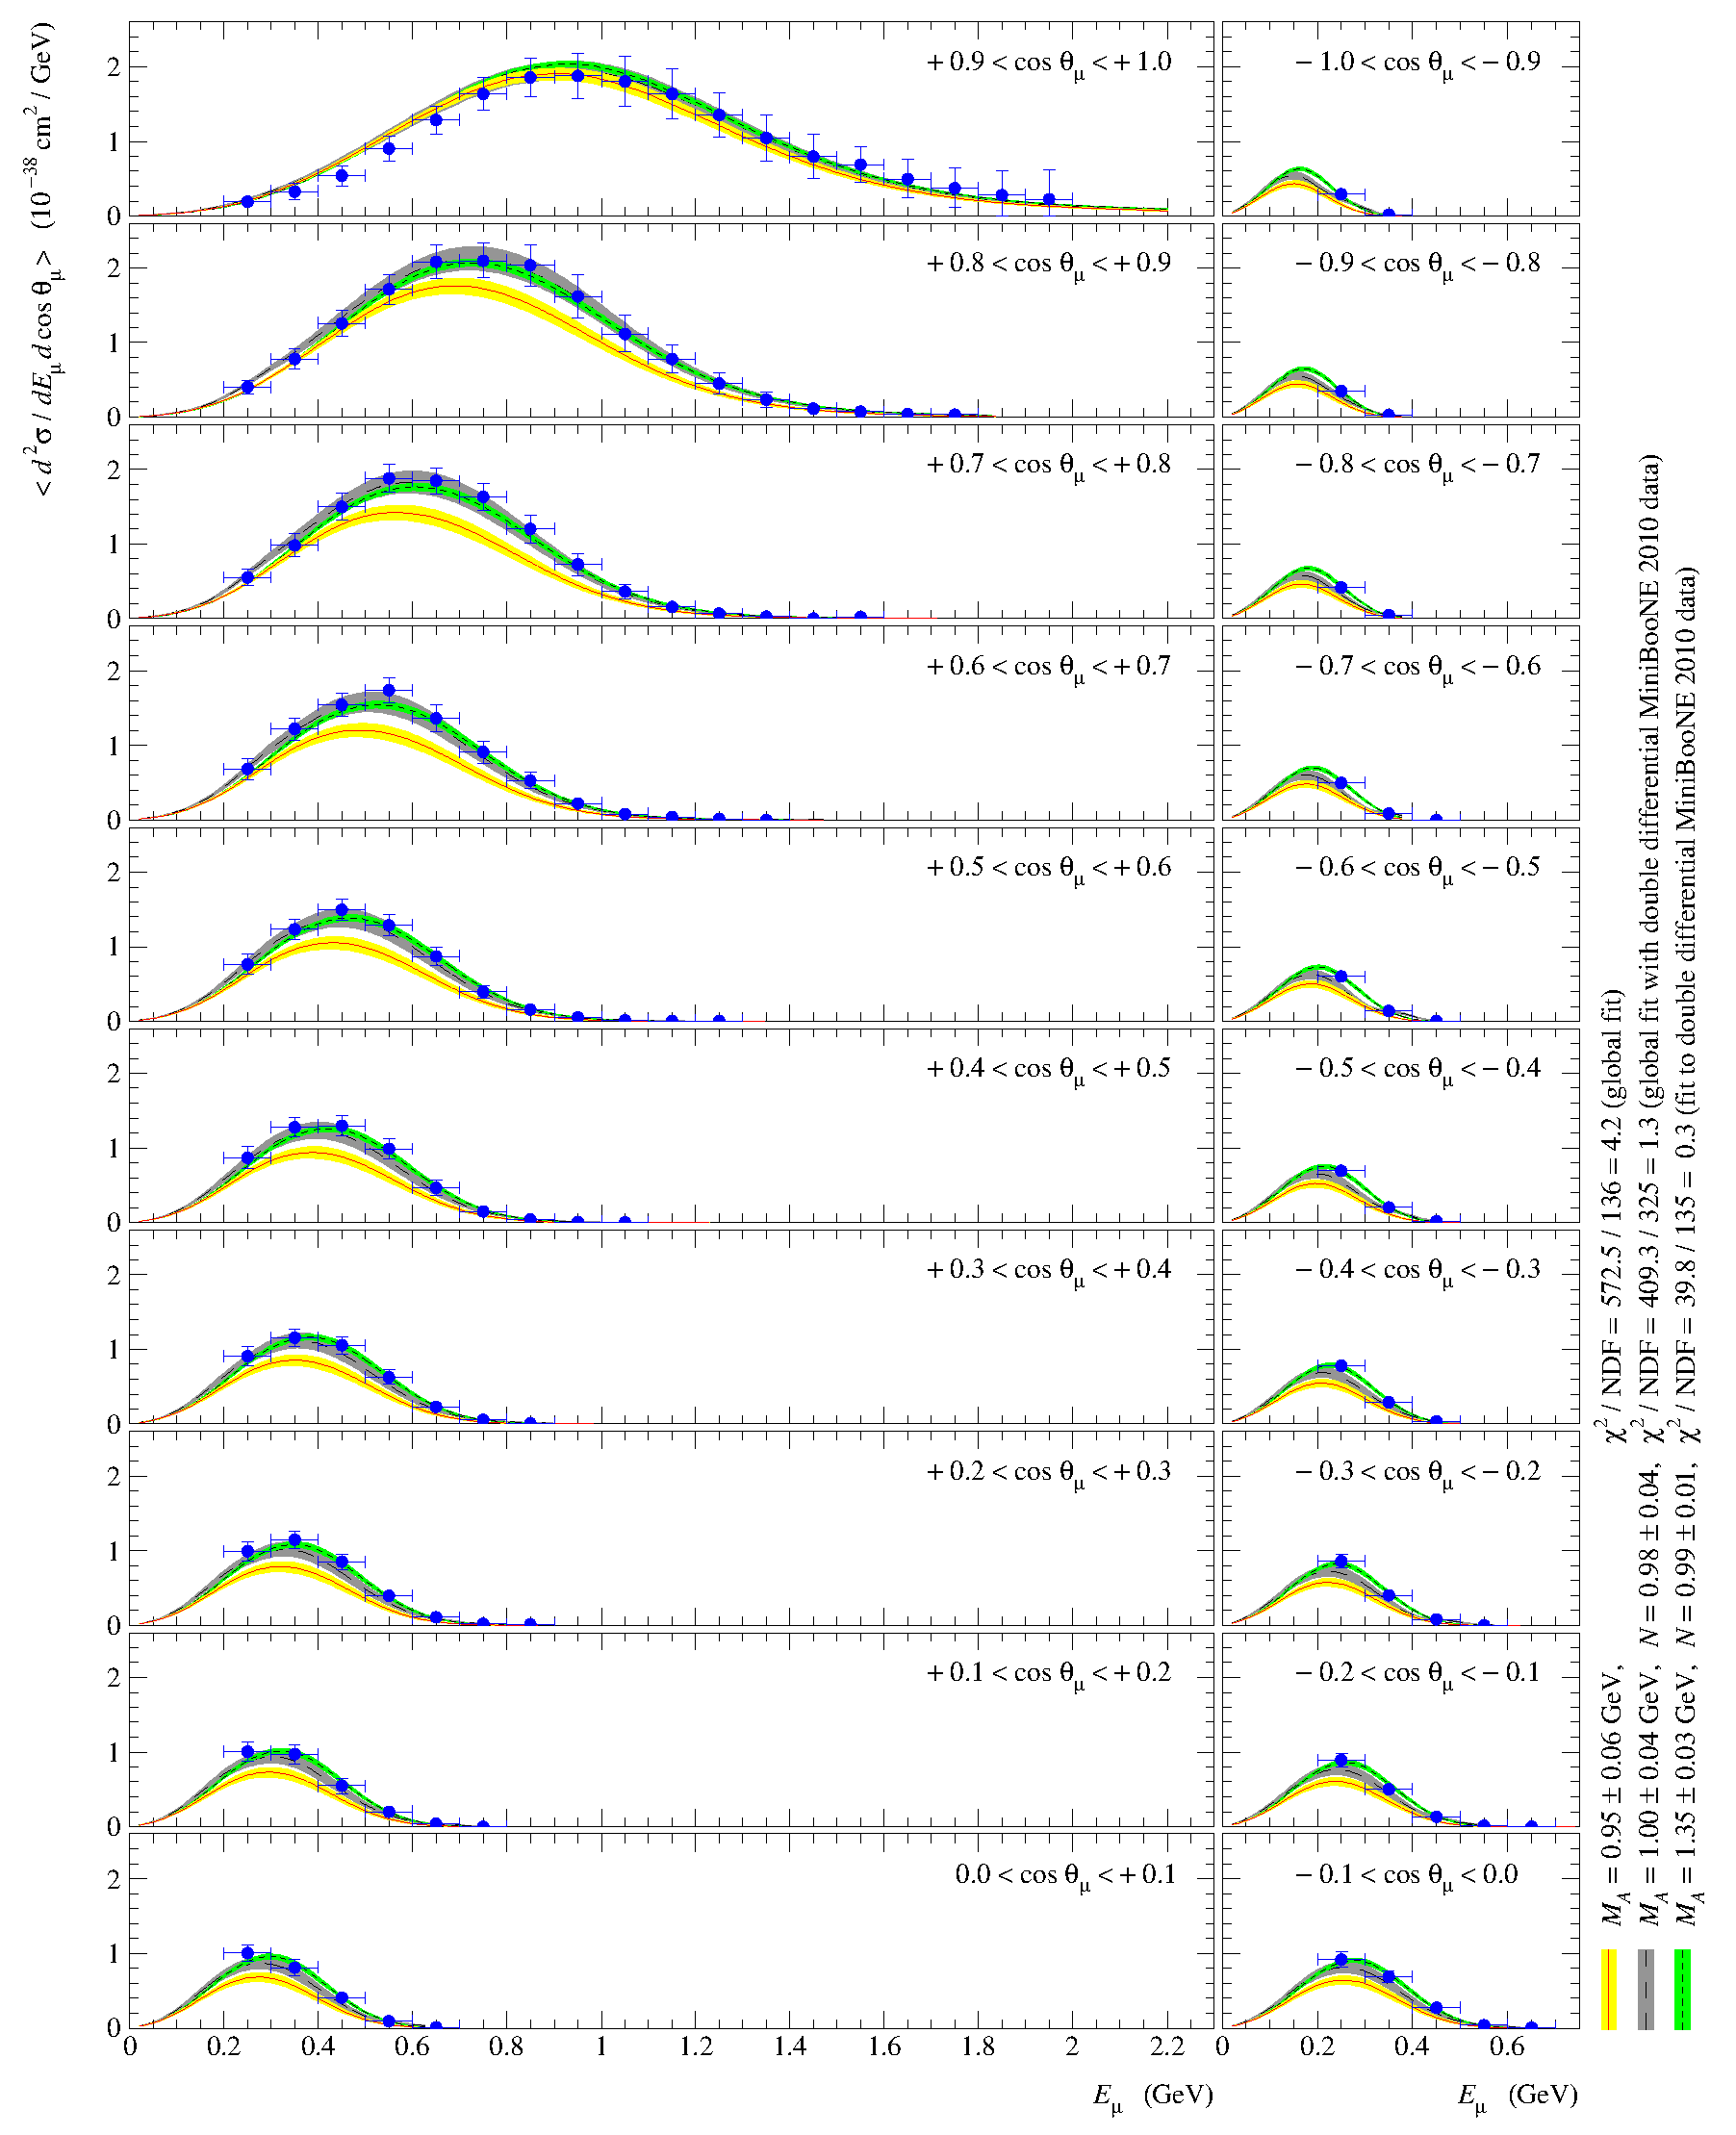
\includegraphics[width=0.5\textwidth]{./QES/d2sQESCC_dEkdcosT_Arevalo_MiniBooNE10_cosT_2_BBBA25.eps}
\caption{\label{MiniBooNE}\textbf{The flux-weighted double differential cross sections} for the $\nu_{\mu}n\to\mu^-p$ reaction measured in the high-statistics experiment MiniBooNE~\cite{AguilarArevalo:2010zc}. The MiniBooNE result: $M_{A}=1.35\pm0.17$\,GeV~\cite{AguilarArevalo:2010zc} is shown by dashed curves corresponding bands. The dark bands are calculated by using the nuclear model of Martini \textit{et al.}~\cite{Martini:2011wp}, \textbf{which yields $M_{A}=1.03$\,GeV} compatible with our best-fit value obtained from high-energy and free-nucleon data}
\end{figure}

Let us stress that the exact knowledge of axial mass is needed for many applications in neutrino physics and astrophysics. In particular, it is important for the data processing of the neutrino oscillation experiments with (anti)neutrinos from accelerators and cosmic rays. The aim of this paper is to investigate the impact of the uncertainty in $M_A$ on the predicted event rates in the underground neutrino detectors. As a major example we consider the World's largest detector Super-Kamiokande.
